\documentclass[12pt]{article}
\usepackage{times}
\usepackage[english]{babel}
\usepackage[utf8x]{inputenc}
\usepackage[colorinlistoftodos]{todonotes}
\usepackage[margin=1in]{geometry}
\usepackage{graphicx}
\usepackage{epstopdf}
\usepackage{cite}
\usepackage{listings}
\usepackage{dtklogos}
\usepackage{wrapfig}
\usepackage{subfigure}
\usepackage{amsmath}
\usepackage{amsthm}
\usepackage{amssymb}
\usepackage{amscd}
\usepackage{caption}
\usepackage{etoolbox}
\usepackage{fancyhdr}
\usepackage{stackengine}
\usepackage[export]{adjustbox}
\patchcmd{\thebibliography}{\section*{\refname}}{}{}{}
\usepackage[document]{ragged2e}    %This causes text to left align
\usepackage[colorlinks=true, linkcolor=black,citecolor=black,urlcolor=blue]{hyperref}
\bibliographystyle{IEEEtran}
\DeclareGraphicsRule{.tif}{png}{.png}{`convert #1 `dirname #1`/`basename #1 .tif`.png}

\title{MCHE 220: Report 1}

\begin{document}
\lefthyphenmin3
\righthyphenmin4
% \pretolerance=2000
% \tolerance=500 
% \emergencystretch=10pt
%\raggedright     %Stops LaTeX from automatically hyphenating the right margin to fit better
%Combine this with \usepackage[document]{ragged2e} to get a text align left similar to natural MS Word
%-------------------------------------------------------------
%Header
%-------------------------------------------------------------
\fancyhf{}  
  \renewcommand{\headrulewidth}{0pt}
  \fancypagestyle{plain}{
    \fancyhead[R]{\thepage}} 
    \pagestyle{plain}
    
\captionsetup[table]{labelsep=space}

\begin{flushleft}
\hrulefill\\\hrule height 1pt
\vspace{5pt}
\textbf{TO: }William J. Emblom, Ph.D.  \hfill   \textbf{DATE: }\today                
\bigskip\\
\textbf{FROM: }Matthew J. Begneaud
\bigskip\\
\textbf{COPY: }N/A
\bigskip\\
\textbf{RE: }MCHE 220 Lab 1
\vspace{-10pt}
\end{flushleft}
\hrulefill \hrule height 1pt

%-------------------------------------------------------------
%Start of Paper
%-------------------------------------------------------------

\section*{\fontsize{12}{12}\selectfont INTRODUCTION}
This memorandum is being sent to Dr. Emblom to convey the analysis of a compression test which took place on campus at University of Louisiana at Lafayette. The test was performed on an aluminum cylinder using a hydraulic press. The results of the test will be shown, as well as multiple plots of various data recorded and calculated from the experiment. These graphs will be used to analyze the meaning of the data.
\bigskip


\section*{\fontsize{12}{12}\selectfont BACKGROUND}
The data collected from the test include forces recorded at various steps of the compression, along with the corresponding length of the cylinder at that time. The original diameter of the cylinder is also recorded. Using the given data, the engineering stress and engineering strain are both calculable. The engineering stress is defined as the force applied to an object divided by the original area of the face the force is applied on, as shown in (1). The engineering strain is defined as the change in length of an object per unit-length, as shown in (2).

\bigskip
\begin{equation}
\sigma = \frac{F}{A_{o}}
\end{equation}
\bigskip

\bigskip
\begin{equation}
\epsilon = \left | \frac{l_{o}-l}{l_{o}} \right |
\end{equation}
\bigskip

Using the given data, the area at any point of the test is also calculable by relating the volume to the change in length and solving for the new corresponding area, resulting in (3). True stress, which is defined as the force applied to an object divided by the current area of the face the force is applied on, is calculable by (4). True strain is also calculable with the given data. According to [1], true strain is found by integrating the rate of the deformation tensor with respect to time, which results in (5).

\begin{equation}
A = \frac{l_{o}}{l}A_{o}
\end{equation}

\begin{equation}
\sigma = \frac {F}{A}
\end{equation}
\bigskip

\begin{equation}
\phi = \left | ln \frac{l}{l_{o}} \right |
\end{equation}
\bigskip

Observing the behavior of both forms of stress and strain can give insight to the properties and behavior of the material used in the compression test.
\bigskip


\section*{\fontsize{12}{12}\selectfont PROCEDURE}
The compression test was conducted in the metal forming lab on campus. The equipment used was a hydraulic press, two cylinders of annealed commercially pure aluminum (AL-1100-O), and oil for lubricating the cylinders. An aluminum cylinder was placed in the hydraulic machine press after recording the original length and diameter of the cylinder. The increase in applied force was periodically stopped in order to record the current force and length. After the data was collected, it was placed in an excel worksheet and converted to metric units. Calculations gave information such as the original area, intermediate areas, engineering stress and strain, and true stress and strain.
\bigskip

The force was plotted against the displacement (change in length) of the cylinder and a trend-line was fitted to the plot. The engineering stress was plotted against the engineering strain, as well as the true stress vs the true strain, on a log-log graph. The true stress was then plotted against the true strain again on a log-log graph and fitted with three different types of trend-line: linear, power, and exponential.
\bigskip


\section*{\fontsize{12}{12}\selectfont RESLTS AND DISCUSSION}
The data recorded from the experiments is plotted and is shown in Table 1. A plot shows how the force placed on the cylinder correlated to the compressive displacement in Figure 1. This data is fitted with two trend lines to estimate the behavior of the material. One trend line shows a linear curve fit, which clearly shows the relationship of the force and displacement is not linear. The other trend line shows a third degree polynomial fit, which matches the data curve quite well. From this, we can gather that the behavior of the material is seemingly cubic when considering force versus displacement.

\newpage

% table1
\begin{center}
Table 1 
\\
\emph{Compression of Aluminum (AL-1100-O)}
\\
\bigskip
\begin{tabular}{ c c c c c c c }
\hline
Force & Length & Area & Engineering Stress & Engineering Strain & True Stress & True Strain\\
(kN) & (mm) & (mm$^2$) & (MPa) & --- & (MPa) & ---\\
\hline
0 & 27.609 & 503.123 & 0 & 0 & 0 & 0\\
37.921 & 25.908 & 536.156 & 75.375 & 0.0616 &  70.727 & 0.0635\\
53.618 & 23.419 & 593.139 & 106.570 & 0.1517 & 90.397 & 0.1645\\
69.121 & 20.955 & 662.883 & 137.384 & 0.2410 & 104.273 & 0.2757\\
87.612 & 18.542 & 749.149 & 174.136 & 0.3284 & 116.948 & 0.3981\\
110.96 & 16.052 & 865.358 & 220.542 & 0.4185 & 128.224 & 0.5423\\
143.895 & 13.640 & 1018.381 & 286.004 & 0.5059 & 141.297 & 0.7051\\
191.722 & 11.252 & 1234.511 & 381.064 & 0.5924 & 155.301 & 0.8975\\
269.904 & 8.991 & 1544.959 & 536.457 & 0.6743 & 174.699 & 1.121\\
394.423 & 6.909 & 2010.526 & 783.949 & 0.7497 & 196.179 & 1.385\\
\hline
\end{tabular}
\end{center}

% figure1
\begin{figure}[h!]  
  \centering
    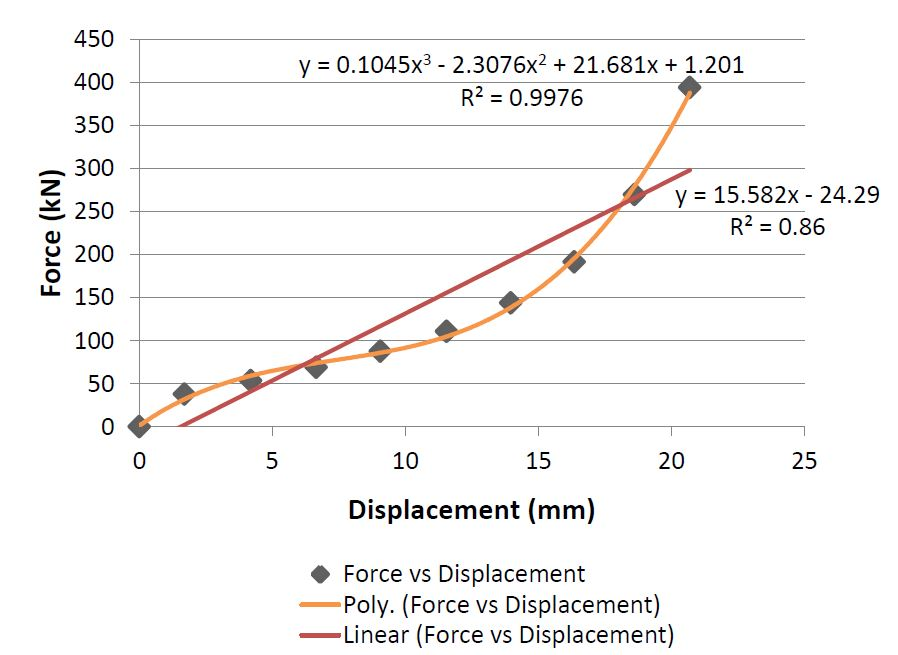
\includegraphics[width=\linewidth]{force_vs_displacement.JPG}
    \caption{Force vs Displacement}
\end{figure}

\newpage

The engineering stress and strain, as well as true stress and strain, are plotted to show the correlation of the stress and strain in the cylinder. As shown in Figure 2, the engineering stress and strain behave quite differently than the true stress and strain after passing the yield point of the material. This is most likely due to the fact that engineering strain does not account for the change in area of the cylinder as it compresses. Since only the original area is considered in the engineering strain, the area does not increase as it does in reality, which results in a higher-than-realistic stress calculation for compression (for a material under tension, the stress would be underestimated rather than overestimated). True stress considers the change in area as the cylinder compresses [2], which results in a more linear behavior, as shown in Figure 2.
\bigskip
\bigskip
\bigskip
\bigskip

% figure2
\begin{figure}[h!]  
  \centering
    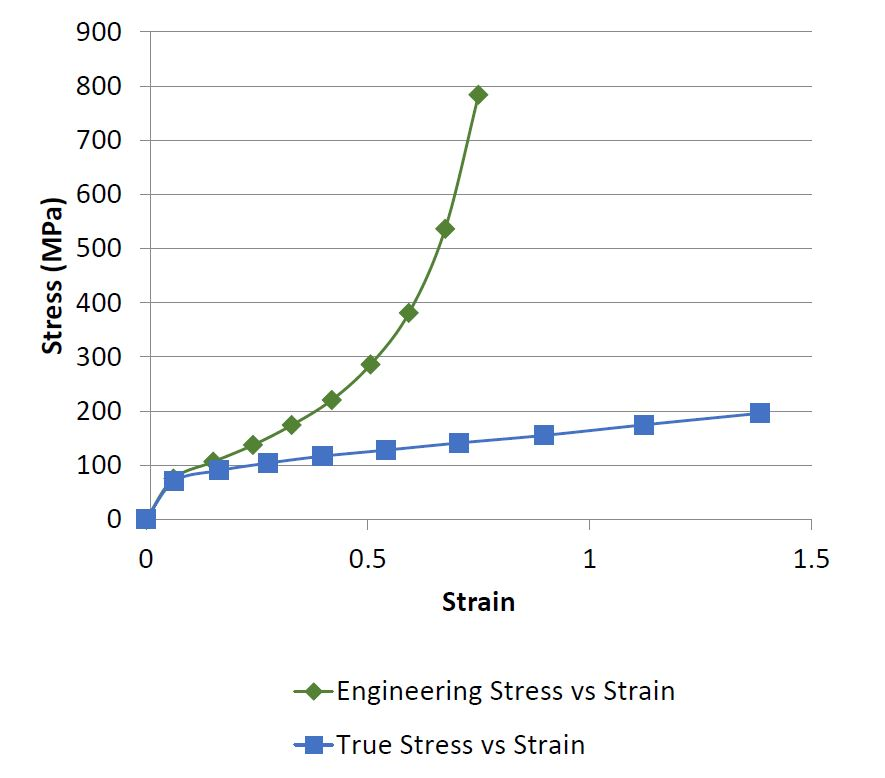
\includegraphics[width=\linewidth]{stress_vs_strain.JPG}
    \caption{Stress vs Strain}
\end{figure}

\newpage

When the same information from Figure 2 is shown on a log-log scale in Figure 3, it is shown again that the true stress and strain follow a more linear trend than the engineering stress and strain. The plot, however, does not show the behavior near a stress or strain value of zero since zero has no logarithm (i.e. zero does not exist in the logarithmic scale).
\bigskip

The true stress and strain are also plotted on a log-log scale and fitted with trend lines, shown in Figure 4. The three trend lines used are linear, power, and exponential fits. It is seen that the power law trend line fits the data best, and looks linear in a log-log scale. This is because the slope for the power law curve is expressed as an equation consisting solely of logarithmic functions, as seen in (6). Since the slope is logarithmic in nature, it appears linear on a log-log scale.
\bigskip

\begin{equation}
B = \frac{ln\sigma_{1}-ln\sigma_{2}}{ln\phi_{1}-ln\phi_{2}}
\end{equation}

% figure3 
\begin{figure}[h!]  
  \centering
    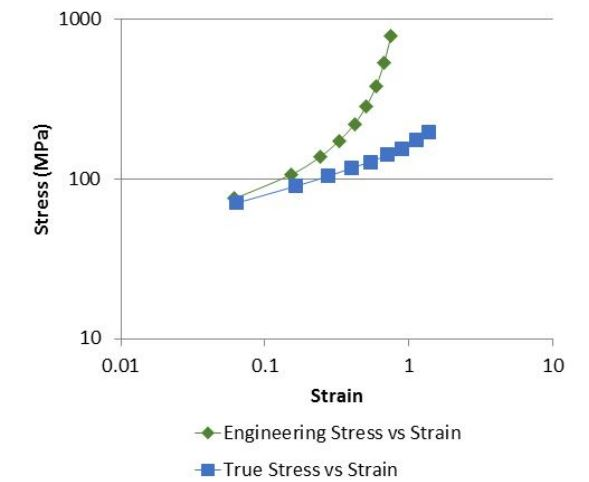
\includegraphics[width=\linewidth]{stress_vs_strain_log.JPG}
    \caption{Stress vs Strain (Log-Scale)}
\end{figure}

\newpage

% figure4
\begin{figure}[h!]  
  \centering
    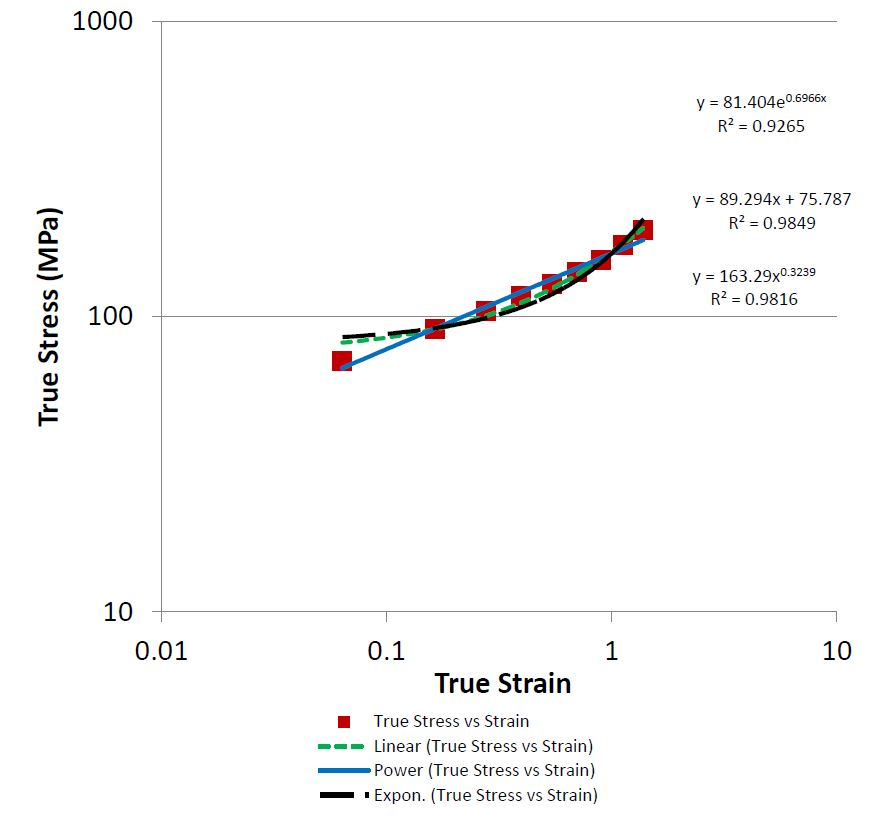
\includegraphics[width=\linewidth]{truestress_vs_truestrain_log.JPG}
    \caption{True Stress vs True Strain (Log-Scale)}
\end{figure}
\bigskip
\bigskip
\bigskip

As discussed, the true stress and strain give more accurate values than the engineering stress and strain. This is because the change in area elements is considered in calculations. Since the two types of stress and strain behave similarly up to the yield point where deformation begins to occur, as shown previously in Figure 2, it is recommended that engineering stress and strain only be used for analysis regarding materials that are not loaded enough to cause any deformation. If deformation is to occur in the range of loading considered for a material, true stress and strain should be used. 

\newpage

\section*{\fontsize{12}{12}\selectfont CONCLUSION}
The data from this compression test, performed on UL campus, has been analyzed and plotted. The originally recorded data was also used to calculate the engineering stress and strain, as well as the true stress and strain. The results were plotted and it was found that true stress and strain tend to follow a power law trend when plotted against each other, which can be seen in Figure 4, where the power law trend-line fits the data best. The data also shows that the true stress was less than the engineering stress, which is due to the fact that true stress involves the instantaneous area of a material during load, while engineering stress only uses the original area. This difference also results in the true strain being bigger than the engineering strain. Thus, it has been concluded that engineering stress and strain should only be used for analysis when the loadings present on an object do not bring the material past its yield point where deformation begins to occur. If the loads on the object cross into the range where deformation occurs, true stress and strain should be used for analysis to achieve accuracy.
\bigskip


\section*{\fontsize{12}{12}\selectfont REFERENCES}

\begin{thebibliography}{2}

\bibitem{McGinty}
Mcginty, B., n.d.,
"True Strain," \emph{Continuum Mechanics}, from
http://www.continuummechanics.org/

\bibitem{}
n.d., “True Stress versus Engineering Stress,” \emph{Engineering Quality Solutions}, from
http://www.eqsgroup.com/all-about-steel/difference-between-true-stress-and-engineering-stress.asp

\end{thebibliography}

%\section*{\fontsize{12}{12}\selectfont APPENDIX}

%\begin{table}[h!]
%  \caption{}
%  \includegraphics[width=\linewidth]{table1.png}
%\end{table}

\end{document}
----------------------------%TEmplates-------------------------------

-------------------------Figure-----------------------

\begin{figure}[h!]  
  \centering
    \includegraphics[width=\linewidth]{**file**}
    \caption{Docking Station}
\end{figure}

---------------------------Table-----------------------
\begin{table}[ht]
\caption{Nonlinear Model Results} % title of Table
\centering % used for centering table
\begin{tabular}{c c c c} % centered columns (4 columns)
\hline\hline %inserts double horizontal lines
Case & Method\#1 & Method\#2 & Method\#3 \\ [0.5ex] % inserts table
%heading
\hline % inserts single horizontal line
1 & 50 & 837 & 970 \\ % inserting body of the table
2 & 47 & 877 & 230 \\
3 & 31 & 25 & 415 \\
4 & 35 & 144 & 2356 \\
5 & 45 & 300 & 556 \\ [1ex] % [1ex] adds vertical space
\hline %inserts single line
\end{tabular}
\label{table:nonlin} % is used to refer this table in the text
\end{table}



probably best to insert as an image from excel

\bigskip\\
\begin{table}[h!]
  \caption{}
  \includegraphics[width=\linewidth]{**file**}
\end{table}
\bigskip\\





-----------------------------Equations------------------------
-----------------------------Regular
\begin{equation}
a = b + c
\end{equation}

--------------------------------- Multiline
\begin{multline}
a = b + c + d + e + f
+ g + h + i + j \\
+ k + l + m + n + o
\end{multline}

-------------------------------Citations-------------------------
\bibitem{Author last name}
  Last, First., year of publication,
  article name, book(etc) name, from \\
  link goes here

----------------------------------other-----------------------------

equations:
http://moser-isi.ethz.ch/docs/typeset_equations.pdf

citations:
http://library.missouri.edu/engineering/about/guides/asme
https://www.asme.org/shop/proceedings/conference-publications/references